% 
%  chapter2.tex
%  ThesisISEL
%  
%  Created by Matilde Pós-de-Mina Pato on 2012/10/09.
%
\chapter{State of the Art}
\label{cha:users_manual}

Firstly, on section \ref{sec:related_work}, will be made an overview on previously developted work made on this subject, then, on section \ref{sec:async_concepts}, will be made a characterization of the key concepts related to it. By last, on section \ref{sec:state_of_the_art}, are presented and explained several technologies representative of the state of the Art on asynchronous data flux in different programming realities, e.g. on Kotlin, JAVA and C\#. 


% ================
% = Related work =
% ================
\section{Background} % (fold)
\label{sec:related_work}

% Initially, when computers had a single processing unit, the networks only allowed the exchange of few bytes per second and the data servers didn't had the responsiveness requirements that are mandatory today; software computational systems were simpler, in the sense that operations were mostly made in a single execution thread. 
% The servers design, were made without many concerns about availability under demand pressure or computer resource optimization. 
% Consequently, operations that required intensive IO interactions or data request from an external sources, were mostly blocking, non-flexible in terms of responsiveness and interoperability. 

From the end of 80´s to the beginning of the 2000´s, with the acceleration of Moores´s Law in hardware and network bandwidth development, the creation of the web as we know today through the wide spread of use of the HTTP protocol and the support from new operative systems to multithreading support, the necessity of high responsiveness servers started to grow. This increase in demand of new ways to handle data through parallelism, caused the necessity of design new programming models compatible with concurrent work. 

Taking the wave initiated by the Gang of Four in \cite{gof}, where 23 patterns were compiled to deal with object-oriented problems, a group of researchers published the \textit{Proactor Pattern} in the paper \cite{proactor} to deal with asynchronous IO. 
In the document, are identified four properties that high-performance web server must have: 
\begin{itemize}
	\item Concurrency - The server must process multiple client requests simultaneously.\\
	\item Efficiency - The software design must be built aiming the use of least hardware resources as possible. \\
	\item Simplicity - The code of the solution must be easy to understand, modular and avoid own built design patterns as possible. \\
    \item Adaptability - The system must be totally decoupled from client implementations, allowing it to be easily used by any client independently of the underlying technologic realities. To achieve this, may be used standards e.g. \cite{REST} or SOAP.\\
\end{itemize}

The authors propose the \textit{Proactor Pattern}, because in their opinion, conventional concurrency models fail to fully achieve the enumerated properties. In the paper, before presenting the \textit{Proactor Pattern}, are identified two major concurrency models, namely: \textit{multithreading} and \textit{reactive event dispatching}. 

The paper refers that one of the most direct implementations of the multithreading approach, is the handling of multiple requests by creating a new thread every request. Each request will then be fully processed and the recently  created thread is then be disposed after the work is finished. 

This solution has several serious issues. Firstly, creating a new thread per request is highly costly in terms of computational resources,
because are involved context switches between user and kernel modes; secondly, must be taken in account synchronization to maintain data integrity.
Then, the authors warn about the fact that the IO retrieved data is mainly memory-mappped, wich rises the question: What happens when the data obtained through IO becomes greater than the system memory can hold? The system stalls until more memory becomes available!?
On last, if the server receives a high demand of requests, the server easily blocks in the process of creating and disposing threads. 

To avoid this issue, the authors, recommended the use of dynamic threadpools to process requests, where each request will be linked to a pre-existing thread, avoiding all the overhead of creating and disposing a thread per request;
however, issues related with memory-mapping and overhead due to the switching of data between different threads maintains. 

Another traditional concurrency model identified by the authors of the paper, is the \textit{Reactive Synchronous Event Dispatching} or more commonly known as \texttt{Reactor Pattern}. In this model, a \textit{Dispatcher}, with a single thread in a loop, is constantly listening requests from clients and sending work requests to an entity named \textit{Handler}. 
The \textit{Handler}, will then process the IO work Synchronously and request a connection to the client in the \textit{Dispatcher}. When the requested connection is ready to be used, the \textit{Dispatcher} notifies the \textit{Handler}. After the notification, the \textit{Handler} asynchronously sends the data, that is being or has been obtained through IO, to the client.\\
Although the authors identifying that this approach is positive, because decouples the application logic from the dispatching mechanisms besided with the low overhead due the use of a single thread, the authors identify several drawbacks with this approach. 
Firstly, since IO operation are synchronous, the code for this approach is complex because must be set in place mechanisms to avoid IO blocking through hand off mechanisms. 
Then, if a request processing blocks, the processing of another requests may be impacted. 

To keep the positive points but mitigating the identified issues of previous approaches, is suggested the \textit{Proactor Pattern}. 
This pattern is very similar to the \textit{Reactive Synchronous Event Dispatching}, however, after the requests processed by a single threaded \textit{Completion dispatcher}, 
the IO work is then dispatched asynchronously to the underlying OS IO subsystems, where multiple requests can be processed simultaneously. 
For the result to be retrieved, is previously registered a callback in the \textit{Completion Dispatcher} and the OS has the responsibility to queue the finished result in a well known place. 

Finally, the \textit{Completion Dispatcher} has the responsibility to dequeue the result placed by the OS and call the correct previously registered callback. 
With this, this model creates a platform that provides: decoupling between application and processing mechanisms,
offers concurrent work without the issues inherent with the use of threading mechanisms and since IO is managed by the OS subsystems, is avoided code complexity in handling possible blocking and scheduling issues.  

The \textit{Proactor Pattern}, creates the ground for several models used by modern platforms that use a single/few threads to process client requests and parallel mechanisms to do the heavy work in the background; namely, for example: \textit{Javascript NODE.JS}, \textit{Spring Webflux}, \textit{vertx} and others.

From what was explained until now, is evident the tendency followed by software architects in terms of asynchronous processing from non-reactive to event driven approaches. Initially the systems were non-reactive, where each request had to be processed in a 
specific thread and that thread blocked until something got ready to go further. 
Then, with the asynchronous systems based on events with the introduction of callback systems inspired in patterns like the \textit{Reactor} or \textit{Proactor}; the software design started to become more event driven, allowing the servers to be more efficient in responsiveness, flexibility and resources optimization. 

However, are some limitations in these asynchronous models. For example, if the data to be processed is bigger than the memory available or if the data to be calculated is from a source that produces data at a constant rate that must be processed in real time, these models work badly.  
The traditional models fail to comply these objectives because are mostly eager by design or not comply with the notion of a continuous source of information that requires to be processed in real time.
Taken this in account, projects like project Reactor, Asynchronous Enumerable provided by Microsoft or papers like \cite{LAZYVSEAGER}, try to deal with these issues, by providing API's that merge the concepts of Fluent API´s, functional programming and code syntax that tries to resemble synchronous code, being the complexity inherent with asynchronous models implementations hidden from the programmer. 

%\begin{figure}[ht]
%	\centering
%	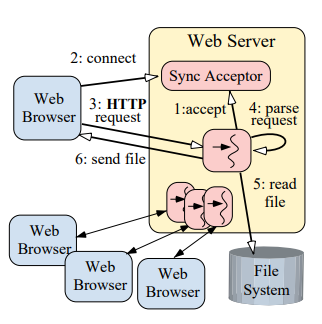
\includegraphics[width=0.65\textwidth]{alternative_1}
%	  \caption{Multithreading solution example}
 % \label{fig:bibtex}
%\end{figure}


%\begin{figure}[ht]
%	\centering
	%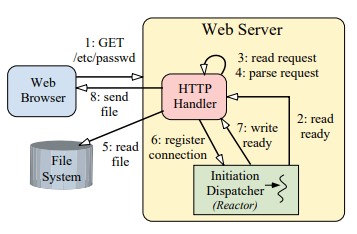
\includegraphics[width=0.65\textwidth]{alternative_2}
%	  \caption{Dispatcher example}
 % \label{fig:bibtex}
%\end{figure}

%\begin{figure}[ht]
%	\centering
%	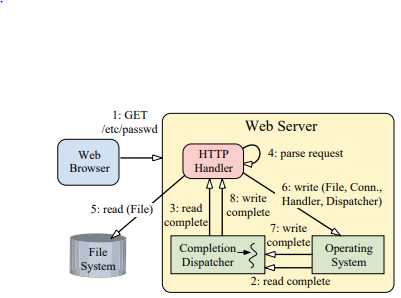
\includegraphics[width=0.65\textwidth]{alternative_3}
%	  \caption{Proactor example}
%  \label{fig:bibtex}
%\end{figure} %

% section introduction (end)

% ====================
% = Folder Structure =
% ====================
\section{Asynchronous flux key concepts and design alternatives} % (fold)
\label{sec:async_concepts}

With the development of several approaches and implementations related to asynchronous data flux in several programming plataforms; a dictionary
of properties, concepts and design alternatives started to grow by itself. In the following, are discussed several of the concepts related with asynchronous data flux, namely:


\subsection{Synchrony versus Asynchrony}

	Before explaining more terms related with asynchronous data flux, it's important to clarify what is synchrony and asynchrony in programming. 
	
	Asynchrony in programming, is a call to a function or routine that returns immediately, not blocking the caller until the operation is finished. The operation processing, will be completely independent from the caller execution thread and can even be done in another machine and technology. This way, the caller is freed to do more work, even to start \texttt{N} more operations in parallel. 
	
	Meanwhile, a call to a synchronous function or routine, blocks the caller until the operation finishes. In this case, the caller has to wait for the completion of the synchronous call before going forward, which limits the program efficiency if parallelism is applicable.
	Usually, in this case, the execution \texttt{Thread} of the caller is 

	To better visualize what was explained, we have the following example: 


	\begin{figure}[htbp]
		\centering
		\begin{subfigure}[h]{0.4\textwidth}
			\centering
			\lstfromfile{java}{1-8}{Asynchronous call example}{async}{showlines=true,morekeywords={begin,System,out,print},numbers=left, firstnumber=1}{async.java}
			\caption{}
			\label{fig:ra-vectorial}
		 \end{subfigure}	
	\qquad
		 \begin{subfigure}[h]{0.4\textwidth}
			\centering
			\lstfromfile{java}{1-8}{Synchronous call example}{Sync}{showlines=true,morekeywords={begin,System,out,print},numbers=left, firstnumber=1}{Sync.java}
			\caption{}
			\label{fig:ra-raster}
		\end{subfigure}		
	  \caption{Example of Synchronous and Asynchronous calls in JAVA}
	  \label{fig:figura-completa}
	\end{figure}

	As we can see, in the synchronous call example, the operation return only happens after the whole subsequent operation is finished, consequently, the print of the message made in the synchronous routine happens right before the second statement call. 

	Meanwhile, in the asynchronous operation call, the return happens immediately after the call, however, the processing inherent with that operation will start just when the subsystem that handles the asynchronous function is ready to process that work, for example, when a worker thread from a threadpool is ready to handle that work.
	Because of that, the print made in the asynchronous operation will happen "out of order", being done just after the print of the second statement.




	\subsection{Push vs Pull} 
	
	Another concept important to understand how asynchronous data flux is handled in programming, is the \textit{Pull} and \textit{Push} processing patterns.
	In \textit{Pull} pattern, usually, exists a source of data and the program iterates over that source to operate over each item. 
	
	On the other hand, in the \textit{Push} pattern, the items of the data source are "Pushed" to a routine that will operate over that item.
	To help to assimilate what was just explained, we have the following example:

	\begin{figure2}
		\centering
		\begin{subfigure}[h]{0.4\textwidth}
			\centering
			\lstfromfile{java}{1-13}{Pull pattern example}{pull}{showlines=true,morekeywords={begin,System,out,print},numbers=left, firstnumber=1}{pull.java}
			\caption{}
		 \end{subfigure}	
	\qquad\qquad
		 \begin{subfigure}[h]{0.4\textwidth}
			\centering
			\lstfromfile{java}{1-13}{Push pattern example}{push}{showlines=true,morekeywords={begin,System,out,print},numbers=left, firstnumber=1}{push.java}
			\caption{}
		\end{subfigure}		
	  \caption{Example of Pull and Push data handling patterns}
	  \label{fig:exmplo2}
	\end{figure2}
	
	As we can see, in the pull pattern, the items are "pulled" from a data source through an iteration mechanism. 
	
	In contrast with that, in the \textit{Push} pattern, items are pushed to a consumer through a supplier.





	\subsection{Hot versus Cold}
	
	Another property that must be took in account when handling this subject is nature of a data flux. There are two main adjectives to name a data flux, Hot or Cold.  \\

	A cold data flux, is a sequence of information that is received by a consumer with the control of that consumer. 
	For example, when program uses a stream to lazily retrieve a sequence of words from a buffer, the consumer has total control on when and how the next item will be proccessed.

	On the other hand, in a \texttt{Hot} data flux, the consumer has no control on how many items will receive in the given moment. 
	In a Hot data flux, the consumer can receive data from the moment the stream is open while in a Cold stream, the consumer will receive just when data is requested from the stream.

	\begin{figure3}
		\centering
		\begin{subfigure}[h]{0.4\textwidth}
			\centering
			\lstfromfile{java}{1-3}{Cold Example}{cold}{showlines=true,morekeywords={begin,System,out,print},numbers=left, firstnumber=1}{ColdFlux.java}
			\caption{}
		 \end{subfigure}	
	\qquad\qquad
		 \begin{subfigure}[h]{0.6\textwidth}
			\centering
			\lstfromfile{java}{1-6}{Hot Example}{hot}{showlines=true,morekeywords={begin,System,out,print},numbers=left, firstnumber=1}{HotFlux.java}
			\caption{}
		\end{subfigure}		
	  \caption{Example of Hot and Cold data streams}
	  \label{fig:exmplo3}
	\end{figure3}

	As we can see, in the \texttt{Hot} data flux example, the items are emitted from the moment the emitter is created. 
	In the example, the emitter emits a number per hundred milliseconds, where the number is 1 or the "repetition number" + 1. Since the stream is continuous, when the consumer starts to listen the pipepline 1 seconds after the emittion started, 10 items were already lost when a observer subscribes to that data source.
	However, in the \texttt{Cold} example, the consumer only receives the items when he manually consumes the pipeline.

	%\subsection{Cancelables} \\
	%\subsection{Error Handling}  \\
	%\subsection{Intrisic Keywords} \\
    %\subsection{Reactive Streams} \\
	%\subsection{Async Enumerables} \\ 

    

% The template file for writing dissertations in  \texttt{LaTeX} is organized into a main directory, a set of files and sub-directories:
% \begin{enumerate}
% 	\item[ThesisISEL] This is the main directory and includes:
% 	\begin{enumerate}
% 		\item \textbf{Logo} Directory with Faculty logos;
% 		\item \textbf{sty} Directory will all sty files that help in formatting document;
% 		\item \textbf{Chapters} Directory where to put user files (text and figures);
% 		\begin{enumerate}
% 		\item \textbf{scripts} Directory with useful bash scripts, e.g., for cleaning all temporary files;
% 		\item \textbf{img} Directory with all images of your thesis;
% 		\end{enumerate}
% 		\item \textbf{alpha-pt.bst} A file with bibliography names in portuguese, e.g., 'Relatório Técnico' e 'Tese de Mestrado' instead of 'Technical Report' and 'Master Thesis'. This file is used automatically if Portuguese is selected as the main language (see below);
% 		\item \textbf{defaults.tex} A file with the main default values for the package (institution name, faculty's logo, degree name and similars);
% 		\item \textbf{personaldataofthesis.tex} A file with the main default values for the package (identification of report as well as the author and juries);
% 		\item \textbf{template.tex} The main file. You should run  \texttt{LaTeX} in this one. Please refrain from changing the file content outside of the well defined area;
% 		\item \textbf{bibliography.bib} The bib file. An easy way to find to import citation into \texttt{bibtex} is select option \texttt{Show links to import citation into
% Bib\-Tex} in \href{http://scholar.google.pt/scholar_settings?hl=en&as_sdt=0,5}{\texttt{Scholar google settings}}.
% 		\item \textbf{thesisisel.cls} The  \texttt{LaTeX} class file for the thesis{} style. Currently, some of the defaults are stored here instead of \verb!defaults.tex!. This file should not be changed, unless you're ready to play with fire! :)
% 	\end{enumerate}
% \end{enumerate}

% Again, we would like to recall that all the user \texttt{LaTeX} files should be stored in the \verb!ThesisISEL! directory, and all the images in \verb!ThesisISEL/Chapters/img! directory.\todo[inline]{Yet another note!}
% section folder_structure (end)

% ===================
% = Package options =
% ===================
\section{State of the Art} % (fold)
\label{sec:state_of_the_art}

The thesis{} style includes the following options, that must be included in the options list in the \verb!\documentclass[options]{thesisisel}! line at the top of the \texttt{template.tex} file.

The list below aggregates related options in a single item. For each list, the default value is prefixed with a *.

\subsection{Language Related Options} % (fold)
\label{sub:language_related_options}

You must choose the main language for the document. The available options are:

\begin{enumerate}
	\item \textbf{*pt} --- The text is written in Portuguese (with a small abstract in English).
	\item \textbf{en} --- The text is written in English (with a small abstract in Portuguese).
\end{enumerate}

The language option affects:
\begin{itemize}
	\item \textbf{The order of the summaries.} At first the abstract in the main language and then in the foreign language. This means that if your main language for the document in english, you will see first the abstract (in english) and then the 'resumo' (in portuguese). If you switch the main language for the document, it will also automatically switch the order of the summaries.
	\item \textbf{The names for document sectioning.} E.g., 'Chapter' vs.\ 'Capítulo', 'Table of Contents' vs.\ 'Índice', 'Figure' vs.\ 'Figura', etc.
	\item \textbf{The type of documents in the bibliography.} E.g., 'Technical Report' vs.\ 'Relatório Técnico', 'MSc Thesis' vs.\ 'Tese de Mestrado', etc.
\end{itemize} 

No mater which language you chose, you will always have the appropriate hyphenation rules according to the language at that point. You always get portuguese hyphenation rules in the 'Resumo', english hyphenation rules in the 'Abstract', and then the main language hyphenation rules for the rest of the document. If you need to force hyphenation write inside of \verb!\hyphenation{}! the hyphenated word, e.g. \\
\verb!\hyphenation{op-ti-cal net-works}!.
% section package_options (end)

\subsection{Class of Text} % (fold)
\label{sub:class_of_text}

You must choose the class of text for the document. The available options are:

\begin{enumerate}
	\item \textbf{bsc} --- BSc graduation report.
	\item \textbf{prepmsc} --- Preparation of MSc dissertation. This is a preliminary report graduate students at ISEL/IPL must prepare to conclude the first semester of the two-semesters MSc work. The files specified by 
	\begin{inparaenum}
	\item \verb!\dedicatoryfile! and 
	\item \verb!\acknowledgmentsfile! 
	\end{inparaenum}
	are ignored, even if present, for this class of document.
	\item \textbf{msc} --- MSc dissertation.
\end{enumerate}
%% subsection class_of_text (end)
%
%% ============
%% = Printing =
%% ============
\subsection{Printing} % (fold)
\label{sub:printing}

You must choose how your document will be printed. The available options are:

\begin{enumerate}
\item \textbf{oneside} --- Single side page printing, and
\item \textbf{*twoside} --- Double sided page printing.
\end{enumerate}

The article 50th, of Decree-Law No. 115/2013, requires the deposit of a digital copy of doctoral thesis and master's dissertations in a repository that is part of the RCAAP  repository\footnote{Repositórios Científicos de Acesso Aberto de Portugal}, \url{https://www.rcaap.pt}.  This deposit aims to preserve scientific work, as well as providing Open Access to scientific production is not restricted object or embargo.

For the reason explained above, we include the option to format your thesis in a way that presents well on screen and/or on paper.   But always remember that your work will be stored in the RCAAP portal in electronic format.
% subsection printing (end)

The available options are:

\begin{enumerate}
\item \textbf{onpaper} --- Format your thesis in a way that presents on paper or,
\item \textbf{*onscreen} --- on screen.
\end{enumerate}

% =============
% = Font Size =
% =============
\subsection{Font Size} % (fold)
\label{ssec:font_size}

You must select the encoding for your text. The available options are:
\begin{enumerate}
	\item \textbf{11pt} --- Eleven (11) points font size.
	\item \textbf{*12pt} --- Twelve (12) points font size. You should really stick to 12pt\ldots
\end{enumerate}
% subsection font_size (end)

% =================
% = Text encoding =
% =================
\subsection{Text Encoding} % (fold)
\label{ssec:text_encoding}

You must choose the font size for your document. The available options are:
\begin{enumerate}
	\item \textbf{latin1} --- Use Latin-1 (\href{http://en.wikipedia.org/wiki/ISO/IEC_8859-1}{ISO 8859-1}) encoding.  Most probably you should use this option if you use Windows;
	\item \textbf{utf8} --- Use \href{http://en.wikipedia.org/wiki/UTF-8}{UTF8} encoding.    Most probably you should use this option if you are not using Windows.
\end{enumerate}
% subsection font_size (end)

% ============
% = Examples =
% ============
\subsection{Examples} % (fold)
\label{ssec:examples}

Let's have a look at a couple of examples:

\begin{itemize}
	\item BSc graduation report, in portuguese, with 11pt size and to be printed one sided (I wonder why one would do this!)\\
	\verb!\documentclass[bsc,pt,11pt,oneside,latin1]{thesisisel}!
	\item Preparation of MSc thesis, in portuguese, with 12pt size and to be printed one sided (I wonder why one would do this!). Note that, \verb!pt! is declared by default, so it can be omitted: \\
	\verb!\documentclass[prepmsc,12pt,oneside,latin1]{thesisisel}!
	\item MSc dissertation, in english, with 12pt size and to be printed double sided on screen. Note that, \verb!twoside! and \verb!12pt! are declared by default, so it can be omitted: \\
	\verb!\documentclass[msc,en,utf8,onscreen]{thesisisel}!
\end{itemize}


The present document is defined according to the following settings:
\begin{Verbatim}[breaklines=true, breakanywhere=true]
\documentclass[msc,pt,twoside,12pt,a4paper,utf8,onscreen,hyperref=true,listof=totoc] {thesisisel}
\end{Verbatim}

% subsection examples (end)
	
\section{How to Write Using \texttt{LaTeX}} % (fold)
\label{sec:how_to_write_using_latex}

Please have a look at Chapter~\ref{cha:a_short_latex_tutorial_with_examples}, where you may find many examples of \href{http://tobi.oetiker.ch/lshort/lshort.pdf}{\texttt{LaTeX}} constructs, such as sectioning, inserting figures and tables, writing equations, theorems and algorithms, exhibit code listings, etc.

%% section how_to_write_using_latex (end)
